% This chapter by Robert J. Garner is licensed under a Creative Commons 
% Attribution-NonCommercial-ShareAlike 3.0 Unported License, 
% as described at http://creativecommons.org/licenses/by-nc-sa/3.0/legalcode

To begin learning programming students are often asked to create a simple "hello world" program. In this chapter you will learn the following:


\begin{itemize}
\item Install software needed to write code.
\item Start a new solution/project.
\item Write a simple program (Hello World!).
\end{itemize}

\LevelD{Basic Process}
The basic process for creating a program consists of the following:
\begin{enumerate}
\item Write a program using a text editor.
\item Compile the program using a program called a compiler.
\item Link the program using a program called a linker.
\end{enumerate}
While it is possible to accomplish all of these steps manually, there are programs today called Integrated Development Environments (IDEs) that will handle each of these operations for you and provide an integrated environment to write your code and build it. 

\LevelD{Software Required}
The IDE we will use for this example is a program called Microsoft Visual Studio{TM}. 
You can download a free version from \url{www.visualstudio.com/en-us/products/visual-studio-express-vs.aspx}. 
Alternatively if you are a student you can sign up for a Microsoft DreamSpark account at \url{www.dreamspark.com/}.
Microsoft's DreamSpark{TM} program provides students free access to Microsoft{TM} software. To install the software follow the instructions on the website from which you download it.
 

\LevelD{Working With the IDE}
Once your IDE is installed you should become familiar with the following basic functions:

\begin{itemize}
\item Basic layout of the IDE
\item Opening Windows
\item Re sizing and Moving Windows
\Item Arranging you workspace efficiently
\end{itemize}
\LevelE{Basic layout of the IDE}

Figure 2.1 shows what the Visual Studio interface looks like. If you are familiar with office applications you will recognize several of the menu items such as File, Edit and View. These menus will do much of the same types of functions that they do in other applications. Initially an IDE can be overwhelming to a new programmer because there are many functions and often there are multiple ways of doing the same thing.

\begin{figure}[tb]
  \centering
  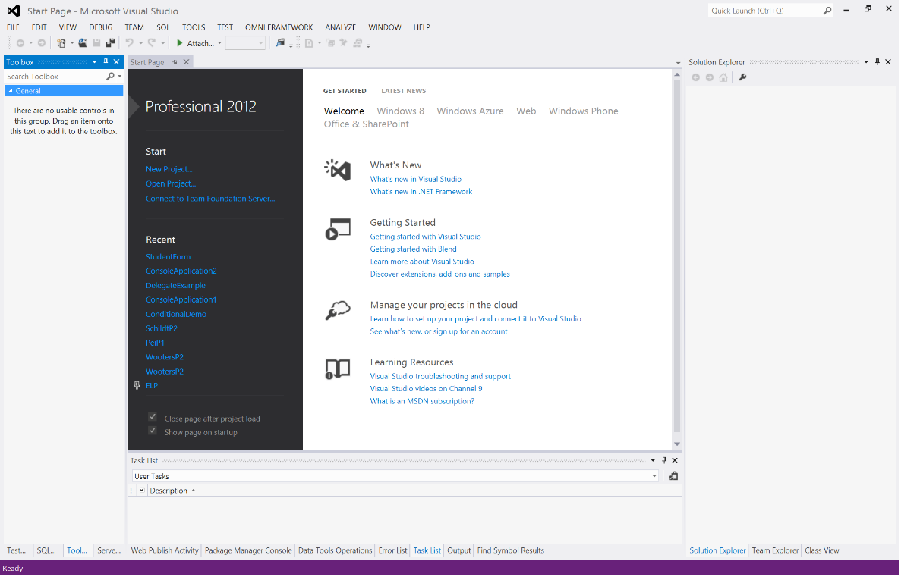
\includegraphics[width=\textwidth]{diagrams/visual_studio_start_page.pdf}
  \caption{Visual Studio Start Page} \label{fig-if-flowchart}
\end{figure}
\LevelD{Creating A New Solution}




